\documentclass[coursework]{SCWorks}
\usepackage{preamble}
% общие настройки для кода
\setminted[python]{fontsize=\footnotesize,baselinestretch=1,linenos,breaklines,frame=single,
    framesep=2mm,numbersep=6pt,tabsize=4,encoding=utf8}
\setminted[cpp]{fontsize=\footnotesize,baselinestretch=1,linenos,breaklines,frame=single,
    framesep=2mm,numbersep=6pt,tabsize=4,encoding=utf8}
\renewcommand{\listingscaption}{Листинг}
\hypersetup{unicode=true,pdftitle={Сравнение линейного и бинарного поиска},
    pdfauthor={Козин Юрий}}

\captionsetup[listing]{hypcap=false}

% титульный лист без блоков руководителей
\makeatletter
\renewcommand{\CDMakeTitle}
{
\thispagestyle{empty}
\shapka
%\vspace{0.5cm}
\begin{center}
%\parbox{8cm}{
%\raggedright
\CYRK\cyra\cyrf\cyre\cyrd\cyrr\cyra\ \@chair
%}
\end{center}

\vspace{14pt}
\vspace{1cm}
{\centering
\textbf{\MakeUppercase{\@title}}
\\[0.3cm]
{\@workname}

}

\vspace{1.5cm}
\begin{flushleft}
\@studenttitle\ \@course\ \cyrk\cyru\cyrr\cyrs\cyra\ \@group\ \cyrg%
\cyrr\cyru\cyrp\cyrp\cyrery\\
\@spectype\ \@napravlenie\\
\@department\\
\@author
\end{flushleft}
\vfill

\vfill
{\centering{\cyr\CYRS\cyra\cyrr\cyra\cyrt\cyro\cyrv\ \@date}

}
\newpage
}
\makeatother


\begin{document}
\title{Сравнение линейного и бинарного поиска}
\course{2}
\group{211}
\author{Козина Юрия}
\chair{математической кибернетики и компьютерных наук}
\department{факультета компьютерных наук и информационных технологий}
\napravlenie{02.03.02 "--- Фундаментальная информатика и информационные технологии}
\date{2026}
\maketitle
\secNumbering
\tableofcontents

\intro
Поиск элемента встречается при работе со списками товаров, книг и учебных
материалов. Один и тот же результат можно получить разными способами,
но количество действий при этом будет различаться.

Цель работы --- сравнить линейный и бинарный поиск в массиве целых чисел.
Для этого рассмотрены правила работы алгоритмов, получены оценки числа
шагов и выполнен небольшой вычислительный эксперимент на Python.

В работе сравнивается число просмотренных элементов, а не время выполнения.
Это позволяет получить воспроизводимый результат, который не зависит
от скорости компьютера. Один шаг означает одну итерацию основного цикла.
При этом внутри шага бинарного поиска может выполняться больше одного
сравнения, поэтому шаги не следует считать одинаковыми по стоимости.

Документ оформлен на основе шаблона СГУ~\cite{sgu}.
Программный код подключён из отдельного файла с помощью пакета
\texttt{minted}, который выполняет подсветку синтаксиса~\cite{minted}.

\section{Описание алгоритмов}
\subsection{Линейный поиск}
Линейный поиск последовательно проверяет элементы массива до обнаружения
нужного значения или до конца массива~\cite{linear}. Предварительная
сортировка для этого не требуется.

Обозначим количество элементов через \texttt{n}, а число шагов линейного
поиска через \texttt{L(n)}. Если значение отсутствует, алгоритм проверяет
все элементы:
\begin{equation}
\mathtt{L}(\mathtt{n})=\mathtt{n}.
\label{eq:linear}
\end{equation}
Если все элементы различны, значение присутствует и каждая его позиция
равновероятна, среднее число шагов равно
\begin{equation}
\overline{\mathtt{L}}(\mathtt{n})=
\frac{1}{\mathtt{n}}\sum_{\mathtt{i}=1}^{\mathtt{n}}\mathtt{i}
=\frac{\mathtt{n}+1}{2}.
\label{eq:average}
\end{equation}
Здесь \texttt{i} --- номер позиции, начиная с единицы.

\subsection{Бинарный поиск}
Бинарный поиск работает с отсортированным массивом. Алгоритм проверяет
середину текущего диапазона и оставляет только ту половину, в которой
может находиться значение~\cite{binary}.

В программе границы диапазона хранятся в переменных \texttt{left}
и \texttt{right}. Индекс среднего элемента \texttt{middle} вычисляется так:
\begin{equation}
\mathtt{middle}=\mathtt{left}+
\left\lfloor\frac{\mathtt{right}-\mathtt{left}}{2}\right\rfloor.
\label{eq:middle}
\end{equation}
Индексы начинаются с нуля. При несовпадении проверенный элемент исключается.

Для непустого массива максимальное число шагов данной реализации равно
\begin{equation}
\mathtt{B}_{\max}(\mathtt{n})=
\lfloor\log_2\mathtt{n}\rfloor+1,\qquad \mathtt{n}\geq 1.
\label{eq:binary}
\end{equation}
Число шагов растёт логарифмически. Формула \eqref{eq:binary}
описывает худший случай; при совпадении поиск заканчивается сразу.


\section{Вычислительный эксперимент}
\subsection{Условия проверки}
Для каждого размера \texttt{n} создаётся список \texttt{data}
из последовательных целых чисел от нуля до \texttt{n - 1}.
Искомому значению \texttt{target} присваивается \texttt{n}.
Такого значения в списке нет, поэтому оба алгоритма должны вернуть
индекс \texttt{-1}. Счётчик \texttt{steps} увеличивается один раз
за итерацию основного цикла.

Полная программа приведена в приложении~\ref{app:source},
в листингах~\ref{code:search} и~\ref{code:experiment}.
Функции возвращают пару: индекс найденного элемента и число шагов.
Для бинарного поиска предполагается, что список уже отсортирован;
затраты на подготовку списка в результаты не включены.

В Python функция \texttt{bisect\_left} модуля \texttt{bisect} использует
похожий принцип, но возвращает позицию вставки. Наличие значения нужно
проверять отдельно~\cite{python}.

\subsection{Полученные результаты}
В таблице~\ref{tab:results} приведены результаты запуска программы.
Для выбранного значения, превышающего все элементы, бинарный поиск
достигает оценки \eqref{eq:binary}.
\begin{table}[H]
\centering
\caption{Число шагов при поиске отсутствующего значения}
\label{tab:results}
\begin{tabular}{|r|r|r|}
\hline
Размер \texttt{n} & Линейный поиск & Бинарный поиск \\
\hline
8 & 8 & 4 \\
16 & 16 & 5 \\
32 & 32 & 6 \\
64 & 64 & 7 \\
128 & 128 & 8 \\
256 & 256 & 9 \\
512 & 512 & 10 \\
1024 & 1024 & 11 \\
\hline
\end{tabular}
\end{table}

На рисунке~\ref{fig:steps} показано изменение числа шагов при увеличении
размера списка. Логарифмическая шкала вертикальной оси позволяет видеть
обе зависимости на одном графике. Графики построены по результатам программы.
\begin{figure}[H]
\centering
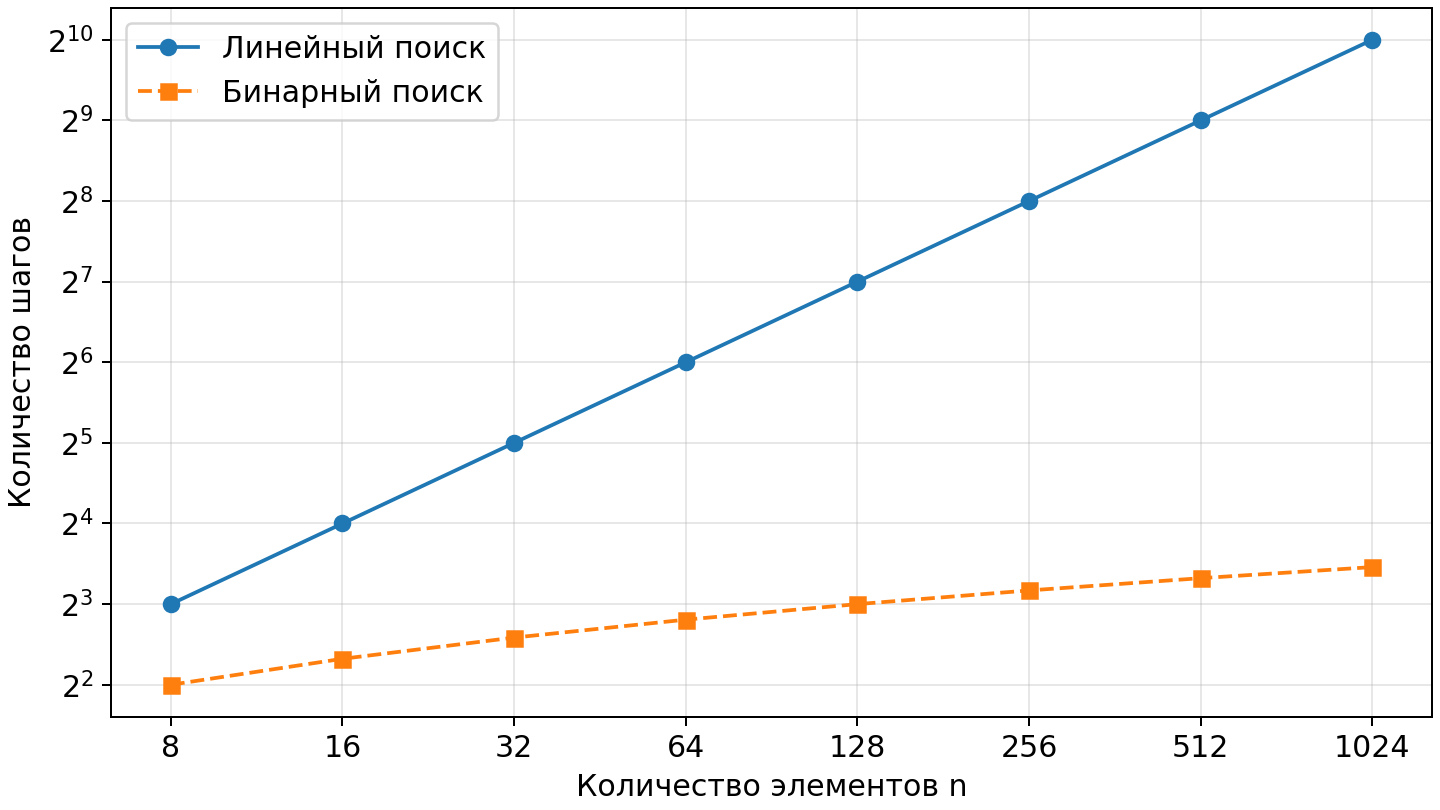
\includegraphics[width=0.82\textwidth]{images/steps.png}
\caption{Число шагов двух алгоритмов}
\label{fig:steps}
\end{figure}

Для сравнения введём отношение числа шагов:
\begin{equation}
\mathtt{K}(\mathtt{n})=
\frac{\mathtt{L}(\mathtt{n})}{\mathtt{B}(\mathtt{n})}.
\label{eq:ratio}
\end{equation}
Здесь \texttt{B(n)} --- число шагов бинарного поиска в эксперименте.
Для размера \texttt{n = 1024} отношение составляет
\(\mathtt{K}(1024)=1024/11\approx 93{,}09\).
Это отношение количества итераций, а не измеренное ускорение программы.

На рисунке~\ref{fig:ratio} видно, как увеличивается отношение
\eqref{eq:ratio}. При переходе от 512 к 1024 элементам линейный поиск
выполняет вдвое больше шагов, а бинарный --- всего на один шаг больше.
\begin{figure}[H]
\centering
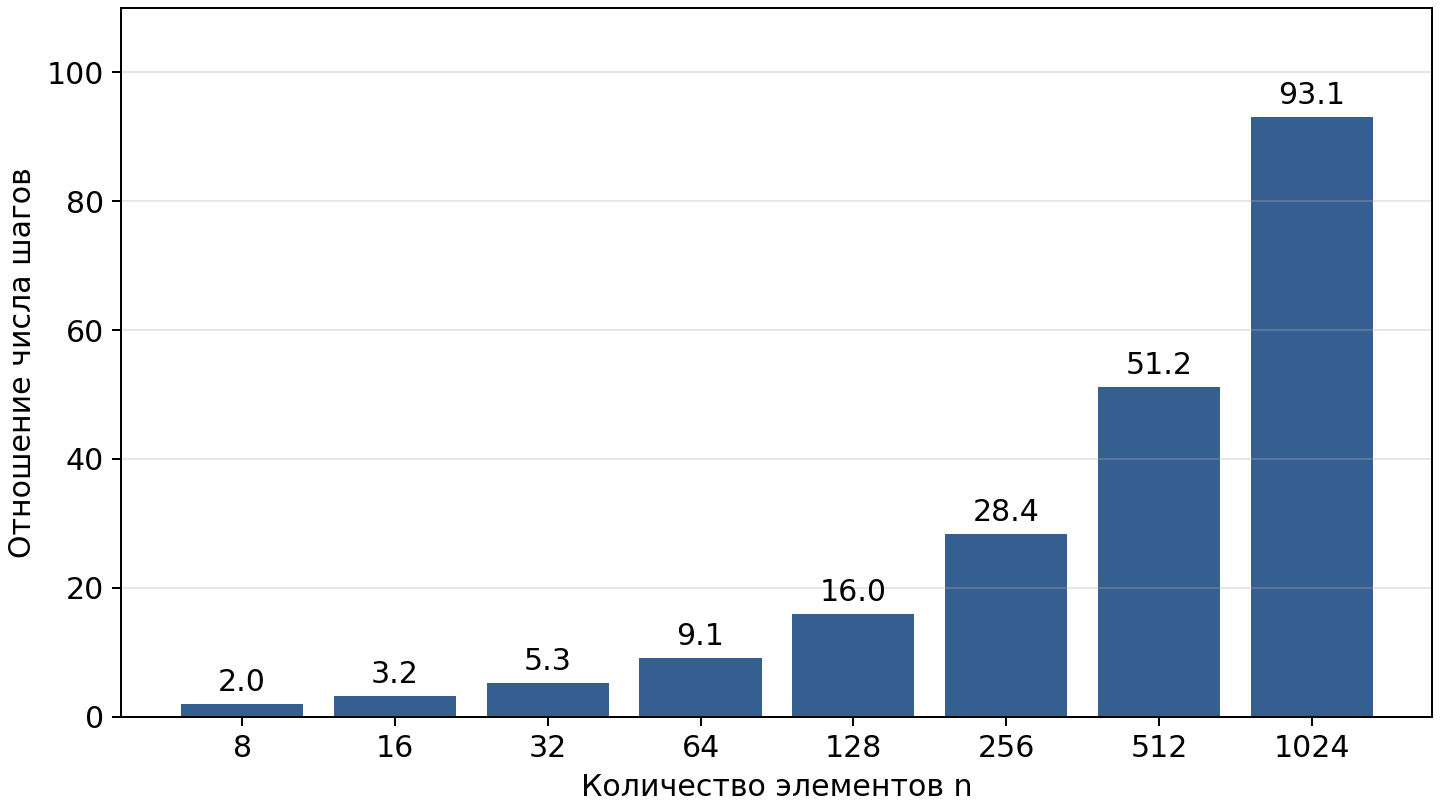
\includegraphics[width=0.82\textwidth]{images/ratio.png}
\caption{Отношение числа шагов линейного и бинарного поиска}
\label{fig:ratio}
\end{figure}

\subsection{Ограничения сравнения}
В опыте рассмотрен один вид запроса: отсутствующее значение больше всех
элементов списка. Для другого запроса количество шагов может измениться.
Например, линейный поиск найдёт первый элемент за один шаг.

Бинарный поиск удобен, когда данные уже упорядочены и обращения по индексу
быстрые. Если требуется только один поиск в неупорядоченных данных,
предварительная сортировка может оказаться лишней работой.
Поэтому результат эксперимента не означает, что бинарный поиск всегда
лучше при любых условиях.

\conclusion
В работе рассмотрены два способа поиска элемента и реализованы их версии
на Python. Для проверки использованы отсортированные списки от 8 до 1024
элементов и отсутствующее значение, превышающее все элементы.

В этих условиях линейный поиск просматривает весь список, а бинарный
последовательно уменьшает диапазон. Для 1024 элементов программа выполнила
1024 шага линейного поиска и 11 шагов бинарного. Результаты согласуются
с полученными оценками.

Линейный поиск проще применять к неупорядоченным данным. Бинарный поиск
требует сортировки, но при многократных запросах к готовому отсортированному
массиву позволяет сократить число просмотров элементов. Выбирать алгоритм
следует с учётом структуры данных и числа запросов.


\bibliographystyle{unsrt}
\bibliography{sources}

\appendix
\section{Исходный код программы}
\label{app:source}
Программа находится в файле \texttt{code/search.py}. Для запуска
из корня проекта используется команда \verb|python3 code/search.py|.
Разделитель столбцов в выводе --- точка с запятой.

\captionof{listing}{Функции поиска}
\label{code:search}
\inputminted[firstline=1,lastline=24]{python}{code/search.py}

\clearpage
\captionof{listing}{Запуск эксперимента}
\label{code:experiment}
\inputminted[firstline=27,firstnumber=27]{python}{code/search.py}

Чтобы пересоздать изображения, можно выполнить
\verb|python3 code/plots.py|. Для этого нужен пакет \texttt{matplotlib}.
Для сборки документа он не требуется: готовые изображения уже находятся
в папке \texttt{images}. Исходный код построения приведён
в листинге~\ref{code:plots}.
\clearpage
\captionof{listing}{Построение графиков}
\label{code:plots}
\inputminted{python}{code/plots.py}

\end{document}
